\documentclass[11pt, luatex, twoside]{book}
\usepackage{chap}


% ============================================================
% БИБЛИОГРАФИЯ (biblatex + biber, стиль ГОСТ)
% ============================================================
\usepackage{csquotes}% нужно для работы biblatex
\usepackage[%
backend=biber,         % движок обработки библиографии
bibencoding=utf8,      % кодировка bib-файла
sorting=none,          % порядок: по порядку цитирования (не по алфавиту)
citestyle=gost-numeric,
bibstyle=gost-numeric, % стиль по ГОСТ
clearlang=true,        % не выводить поле language, если совпадает с~языком документа
]{biblatex}
\addbibresource{lit.bib}               % файл с~библиографической базой
\setlength{\biblabelsep}{4pt}          % отступ от номера в~списке литературы
\AtBeginBibliography{\small}           % уменьшенный шрифт для списка литературы

% -----------------------------------------------------------------------
% Для компиляции одного файла раскомментируй нужную строку:
% \includeonly{chapters/00_frontmatter}
% \includeonly{chapters/01_kinematics_basics}
% -----------------------------------------------------------------------

\begin{document}

% -----------------------------------------------------------------------
% ТИТУЛ
% -----------------------------------------------------------------------
\begin{titlepage}
\thispagestyle{empty}
\vspace*{1cm}

{\headinglight\fontsize{16}{20}\selectfont Крюков П.\,А.}

\vspace{0.5cm}

{\headingfont\fontsize{32}{38}\selectfont Кинематика}

\vfill

\begin{center}
  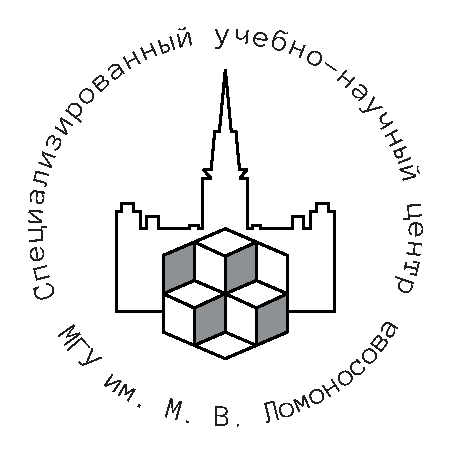
\includegraphics[width=0.6\textwidth]{images/aesc.eps}
\end{center}

\vfill

{\headinglight\fontsize{12}{16}\selectfont \the\year}

\end{titlepage}

% Оборот титула
\thispagestyle{empty}
\vspace*{\fill}
\begin{flushleft}
  \small
  Крюков П.\,А. Кинематика. \\
  \vspace{0.5\baselineskip}
  \textit{Версия от \today.}
\end{flushleft}
\clearpage

% -----------------------------------------------------------------------
% ПРЕДВАРИТЕЛЬНЫЕ СТРАНИЦЫ
% -----------------------------------------------------------------------
\frontmatter
\pagenumbering{arabic}
\section*{Предисловие}
\addcontentsline{toc}{section}{Предисловие}

% Текст предисловия


\section*{Обозначения}
\addcontentsline{toc}{section}{Обозначения}

% Описание пометок и математических обозначений

% Содержит:
%   \section*{Предисловие}
%   \section*{Обозначения}

\tableofcontents
\clearpage

% -----------------------------------------------------------------------
% ОСНОВНОЙ ТЕКСТ
% -----------------------------------------------------------------------
\mainmatter

\chapter{Основы кинематики}

\section{Кинематика одномерного движения}
\subfile{chapters/1D_kinematics}

\section{Относительность движения}
\subfile{chapters/adapted_relative_mov}

\section{Криволинейное движение}
\subfile{chapters/adapted_curve_mov}

\section{Плоскопараллельное движение твёрдого тела}
\subfile{chapters/adapted_pp_moving}

% Содержит:
%   \chapter{Основы кинематики}
%   \section{Относительность движения}
%   \section{Криволинейное движение}
%   \section{Плоскопараллельное движение}

% \include{chapters/02_...}            % пока не готово

% -----------------------------------------------------------------------
% БИБЛИОГРАФИЯ
% -----------------------------------------------------------------------
\backmatter
\addcontentsline{toc}{chapter}{Список литературы}
\printbibliography[]



\end{document}
